% 2011 年辽宁卷文科第 18 题：正方形 ABCD，QA⊥平面 ABCD，PD∥QA。
% 来源 PDF：普通高考/2011/2011辽宁文.pdf，SHA-256 29407891a0a44aaa00db6398312f058fc98c005913323db3729a50333cec4564。
% 原页：第 1 页第 3 栏下部，书页码 683。示意。
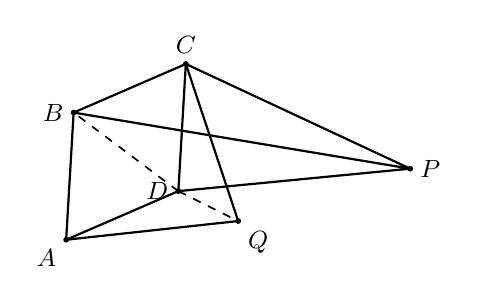
\begin{tikzpicture}[>=stealth, semithick, font=\small, scale=0.95]
  \coordinate (A) at (0,0);
  \coordinate (B) at (0.1,1.7);
  \coordinate (C) at (1.6,2.35);
  \coordinate (D) at (1.5,0.65);
  \coordinate (P) at (4.6,0.95);
  \coordinate (Q) at (2.3,0.25);
  \draw[thick] (A)--(B)--(C)--(D)--cycle;
  \draw[thick] (P)--(D) (P)--(C) (P)--(B);
  \draw[thick] (Q)--(A) (Q)--(C);
  \draw[dashed] (D)--(B) (D)--(Q);
  \fill (A) circle (1.1pt) node[below left] {$A$};
  \fill (B) circle (1.1pt) node[left] {$B$};
  \fill (C) circle (1.1pt) node[above] {$C$};
  \fill (D) circle (1.1pt) node[left] {$D$};
  \fill (P) circle (1.1pt) node[right] {$P$};
  \fill (Q) circle (1.1pt) node[below right] {$Q$};
\end{tikzpicture}
